\htwo{TypeScript}
TypeScript ist eine von Microsoft entwickelte Programmiersprachen, welche auf JavaScript beziehungsweiße, dem ECMAScript-6-Standard basiert. TypeScript unterstützt mithilfe von Modulen das Kapseln von Klassen, Interfaces, Funktionen und Variablen in eigene Namensräume. Dabei wird zwischen internen Modulen, welche sich an den Standard anlehnen und externen Modulen, welche eine JavaScript-Bibliothek wie AMD oder CommonJS verwenden, unterschieden. \cite{TypeScript}

\begin{figure}[H]
    \centering
    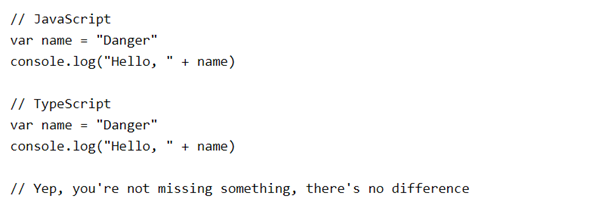
\includegraphics{media/TypeScript/JSvsTS.png}
    \caption{JS vs. TS}
\end{figure}





Aufgrund des Zieles von TypeScript, nur die Erweiterung von JavaScript zu erreichen und beides den gleichen Sprachkern hat, ist der Code derselbe und keine Unterschiede sind bemerkbar. Die Erweiterungen, die von TypeScript erbracht werden, welche Arten von Daten in dem Code verwendet werden, hat also Ähnlichkeiten zu Java. \cite{TypeScript}


\hthree{Problemlösungen mithilfe von TypeScript}
Um sicherzustellen, dass der geschrieben Code keine Fehler enthält, gibt es die Möglichkeit automatisierte Tests anzufertigen und mithilfe dieser manuell zu überprüfen, ob der Code so funktioniert.
Nicht viele Unternehmen haben die Unternehmensgröße von Microsoft, doch sind die meisten Probleme, die bei der Programmierung von Code mit JavaScript auftreten. Große Codebasen bestehen aus mehreren Tausend Dateien. Bei der Änderung eines einzelnen Wertes in einer Datei, kann sich das Verhalten anderer Dateien vollkommen verändern.
Die Validierung von Verbindungen kann schnell zeitaufwendig werden. Eine Sprache wie TypeScript kann dies automatisch erledigen und liefert während der Entwicklung sofortiges Feedback. Mithilfe dieser Funktion, versucht TypeScript Entwicklern mehr Vertrauen in ihren Code zu geben und spart viel Zeit bei der Validierung, um sicherzustellen, dass die Entwickler das Projekt nicht versehentlich beschädigt haben. \cite{ScriptWiki}
